\chapter*{Introduction}
\addcontentsline{toc}{section}{\textit{Introduction}}
\markboth{\textit{Introduction}}{\textit{Introduction}}


\lettrine{\libertineInitialGlyph{V}}{assiliev} invariants are a type of knot invariant that possess special properties among all knot invariants, much like how polynomials are a special kind of function. They fit within a general framework of invariants of topological objects due to Thom, Arnold and Vassiliev. The general theory defines invariants of a class of topological objectss by taking into account not only the objects themselves but also their singular versions and how they all fit within a larger topological space.

The example we discuss in this thesis is that of knots: the space of immersions \({S^{1} \to \mathbb{R}^{3}}\) contains knots (which are the embeddings), but also proper immersions that have one or more intersection points in \(\mathbb{R}^{3}\) and therefore fail to be knots. The singular knots form a space of codimension one within the space of immersions; taking its complement divides the space of immersions into connected components which are exactly the knots. Similarly, inside the space of immersions with one or more intersection points lies the codimension one space of immersions with two or more intersection points, and it again divides up the space of one-singular-point immersions into connected components. This continues, dividing the infinite-dimensional space of immersions into the stratification of the space of knots. A rough schematic illustration of the stratification might look like
\[
	\includegraphics[width=0.5\textwidth, valign=c]{graphics/stratification.pdf}
\]
(but of course this two-dimensional picture doesn't properly represent the infinite-dimensional stratification).

The Vassiliev invariants are functions on the chambers of the strata (the knots) which take into account the walls of the strata by changing by a predictable amount across a wall (or higher-dimensional stratum), therefore obeying a relation between
\[f \left( \double \right) \qquad \text{and} \qquad f \left( \poscross \right) - f\left( \negcross \right).\]

Chapter \ref{ch:vassiliev-invariants-and-chord-diagrams} reviews the theory of Vassiliev invariants, with attention given to the particularly fruitful polynomial analogy. The set of all Vassiliev invariants \(\mathcal{V}\) has the structure of a filtered bialgebra, and its product and coproduct mirror those of the filtered bialgebra of polynomial functions on the real line.

The most important result of the Chapter is the fundamental theorem of Vassiliev invariants, which states that the bialgebra of Vassiliev invariants is effectively described by its associated graded bialgebra \(\mathcal{A}\) of chord diagrams. Once again, this fits neatly into an analogy with polynomials in which elements of \(\mathcal{A}\) are likened with constants of integration. Indeed, any polynomial function of degree \(m\) on the real line can be constructed as a definite integral of the zero function \(m\) times by making some specific choice of the constant of integration in each of the \(m\) definite integrals. This choice of constants at every stage completely describes the polynomial. An arbitrary Vassiliev invariant is described by the algebra \(\mathcal{A}\) of chord diagrams in an analoous way.

In Chapter \ref{ch:lie-theory-and-jacobi-diagrams}, the structure of the algebra \(\mathcal{A}\) is examined. The relations in this algebra have a Lie algebraic flavour, and as such a classical construction of Bar-Natan takes a metric Lie algebra and produces a functional on \(\mathcal{A}\). By the fundamental theorem of the previous chapter this yields a class of Vassiliev invariants. We showcase this construction by computing, following Yang, the values of the functional associated with the exceptional Lie algebra \(\mathfrak{g}_{2}\) on an infinite family of chord diagrams.

Somewhat surprisingly, not all Vassiliev invariants come from this construction, and a more general construction is required which takes not just Lie superalgebras but Lie algebra objects in arbitrary symmetric monoidal categories. We review a classical theorem of Hinich--Vaintrob that every Vassiliev invariant is recovered by this more general construction from some Lie algebra object in some symmetric monoidal category. However, this result does not shed light on what type of symmetric monoidal category suffices to construct all Vassiliev invariants in this way.

The focus of Chapter \ref{ch:welded-knots-isometry-lie-algebras-and-arrow-diagrams} is welded long knots, a type of two-dimensional knotted object in four-dimensional space. Welded long knots also have a theory of Vassiliev invariants and a corresponding version of \(\mathcal{A}\), known as the bialgebra of arrow diagrams \(\mathcal{A}_{w}\). Just as the structure of \(\mathcal{A}\) is Lie algebraic in nature, in a similar way \(\mathcal{A}_{w}\) has structure reminiscent of the cocommutative Drinfeld double of a Lie algebra. We prove a Hinich--Vaintrob style theorem in the theory of welded long knots. This gives an alternative of a result which follows from the work Bar-Natan--Dancso: that for welded long knots, taking Lie algebra objects in the symmetric monoidal category \(\mathbf{sVect}\) of supervector spaces suffices to construct all Vassiliev invariants.

\section*{Conventions}

All knots are assumed to be oriented and framed unless specified otherwise. Where a statement holds for a knot which is drawn unoriented, it holds for both orientations of that knot.
